%!TEX root = OptimalOffline.tex
%input{Siddhartha}
\begin{theorem}
A transmission policy $\{\textbf{p},\textbf{s},N\}$ is an optimal solution to Problem 1 if and only if it satisfies the following structure.
\label{th_algo1_1}
\begin{align}
&\sum_{i=1}^{i=N}g(p_i)(s_{i+1}-s_i)=B_0; 								&&
\label{claim1}
\\
&\nonumber s_{N+1}-s_1=\mathcal{R}_0, 	  								&&\text{ if } s_1>0 \text{ or }
\\
& s_{N+1}\le \mathcal{R}_0,												&&\text{ if } s_1=0;
\label{claim2}
\\
& \nonumber s_{n+1}=\argmin_{t_i: s_n < t_i \le s_{N+1}} CP(s_n,t_i) 	&&\text{ and }
\\
&p_n=CP(s_{n},s_{n+1});\label{claim3}									&&
\\
&\exists s_j:s_j\in \textbf{s} \text{ and } s_j=Q.						&&
\label{claim4}
\end{align}
for $n=\{ 1,2,..,N\}$.
\end{theorem}
\begin{proof}
The proof consists of establishing both necessary and sufficiency conditions. First we work out the necessary part i.e. a optimal policy $\{\textbf{p},\textbf{s},N\}$ must have the given structure. We prove it by the method of  contradiction. We establish structure (\ref{claim3}) at first. Assume the optimal policy $\{\textbf{p},\textbf{s},N\}$ satisfies Lemmas 1-5 and does not satisfy structure (\ref{claim3}). Specifically, say the policy abides by the  structure (\ref{claim3}) from time $s_{1}$ to $s_n$, for some $n\in \{1,2,..,N\}$ but transmission power right after $s_n$ is not the maximum feasible constant power, i.e.
\begin{align}
p_n>CP(s_n,\tilde{s})\text{ where } \tilde{s}=\argmin_{t_i: s_n < t_i \le s_{N+1}} CP(t_i,s_n).\label{claim3_1}
\end{align}
The maximum energy that can used for transmission from time $s_{n}$ to $\tilde{s}$ is $\left(\ETx(\tilde{s}^-)-\ETx(s_{n}^-)\right)$ by Lemma \ref{lemma_energy_consumed}. If $\tilde{s}<s_{n+1}$, the transmission policy uses $p_n(\tilde{s}-s_{n})$ energy from time $s_n$ to $\tilde{s}$. If $\tilde{s}>s_{n+1}$, the transmission power during time $[s_{n+1},\tilde{s}]$ has to be greater than or equal to $p_n$ in terms of Lemma \ref{lemma_increasing_power}. So the total energy used during period $[s_n,\tilde{s}]$ can be lower bounded by $p_n(\tilde{s}-s_{n})$. But, this energy is always more than the maximum energy available from $s_{n}$ to $\tilde{s}$ because
\begin{align}
&\nonumber\ETx(\tilde{s}^-)-\ETx(s_{n}^-)=CP(s_n,\tilde{s})(\tilde{s}-s_{n})\stackrel{(\ref{claim3_1})}{<}p_n(\tilde{s}-s_{n}).
\end{align}
This violates constraint (\ref{pb1_constraint_energy}) and contradicts the optimality of policy $\{\textbf{p},\textbf{s},N\}$.
 
Moving on to other structures, (\ref{claim1}) must be followed by the optimal policy as it is a constraint to the Problem 1 and (\ref{claim4}) follows from Lemma 5. We are left to prove structure (\ref{claim2}). If $s_1=0$ then $s_{N+1}$ has to be less than or equal to $\mathcal{R}_0$ due to constraint (\ref{pb1_constraint_time}). When $s_1>0$, assume that $s_{N+1}-s_1<\mathcal{R}_0$. Now consider the policy where power vector is given by $\{p_1-\alpha,p_2,..,p_{N-1},p_N+\beta \}$ and the corresponding time vector be given by $\{s_1-\gamma,s_2,..,s_{N},s_{N+1}-\delta\}$, where $\gamma=\dfrac{\alpha}{p_1-\alpha}(s_2-s_1)$, $\delta =\dfrac{\beta}{p_N+\beta}(s_{N+1}-s_N)$ and $\alpha ,\beta$ are small positive constants. This policy finishes before the optimal policy $\{\textbf{p},\textbf{s},N\}$ and hence amounts to a contradiction only if we are able to show that it is feasible. By the definition, $s_{2}$ is the first energy arrival which is on the boundary of energy constraint (\ref{pb1_constraint_energy}) i.e. $U(s_2)=\ETx(s_2^-)$ and $s_{N}$ is the last epoch satisfying this condition. So we can choose arbitrarily small $\alpha ,\beta$ such that this new policy would be feasible with respect energy constraint (\ref{pb1_constraint_energy}). For every $\beta\rightarrow 0^+$ we can find a value of $\alpha$ such that the number of bits transmitted in this new policy remains the same as policy $\{\textbf{p},\textbf{s},N\}$ i.e. equal to $B_0$. So, excluding the common parts in the transmission we can equate
\begin{align}
&g(p_N)(s_{N+1}-s_N)+g(p_1)(s_2-s_1)\nonumber
\\
&=g(p_1-\alpha)(s_2-s_1+\gamma)+g(p_N+\beta)(s_{N+1}-s_N-\delta)\nonumber,
\\
&\implies \delta(p_N+\beta)p_N\frac{1}{\beta}\left(\frac{g(p_N)}{p_N}-\frac{g(p_N+\beta)}{p_N+\beta}\right)\nonumber
\\
&=\gamma(p_1-\alpha)p_1\frac{1}{\alpha}\left(\frac{g(p_1-\alpha)}{p_1-\alpha}-\frac{g(p_1)}{p_1}\right).\label{bits_equal}
\end{align}
$\exists$ $\tilde{p}_N:p_N<\tilde{p}_N<p_{N}+\beta$ and $\tilde{p}_1:p_1-\alpha<\tilde{p}_1<p_{1}$ such that
\begin{align}
&\frac{d}{dp} \frac{g(p)}{p} \bigg{\vert}_{p=\tilde{p}_N}=\frac{1}{\beta}\left(\frac{g(p_N+\beta)}{p_N+\beta}-\frac{g(p_N)}{p_N}\right),\label{diff_1}
\\
&\frac{d}{dp} \frac{g(p)}{p}\bigg{\vert}_{p=\tilde{p}_1}=-\frac{1}{\alpha}\left(\frac{g(p_1-\alpha)}{p_1-\alpha}-\frac{g(p_1)}{p_1}\right)\label{diff_2}.
\end{align}
Substituting (\ref{diff_1}) and (\ref{diff_2}) into (\ref{bits_equal}) we get,
\begin{align}
&\delta(p_N+\beta)p_N\frac{d}{dp} \frac{g(p)}{p}  \bigg{\vert}_{p=\tilde{p}_N}
=\gamma(p_1-\alpha)p_1\frac{d}{dp} \frac{g(p)}{p} \bigg{\vert}_{p=\tilde{p}_1}.\label{bits_equal1}
\end{align}
It can be verified that $g(p)/p$ is decreasing function of $p$. As $\tilde{p}_1<\tilde{p}_N$, equation (\ref{bits_equal1}) implies $\gamma >\delta$. Hence the time for which transmission occurs in the new policy ($s_{N+1}-s_1+\gamma-\delta$) is greater than the old one i.e. $s_{N+1}-s_1$. As $s_{N+1}-s_1<\TRx_0$, we can choose arbitrarily small negative value of $\beta$ so that $s_{N+1}-s_1<s_{N+1}-s_1+\gamma -\delta<\TRx_0$ holds. So the new policy is feasible with constraints  (\ref{pb1_constraint_bits}), (\ref{pb1_constraint_energy}), (\ref{pb1_constraint_time}) and contradicts the optimality of policy $\{\textbf{p},\textbf{s},N\}$. This concludes that $s_{N+1}-s_1=\TRx_0$ (if $s_1\neq 0$) in optimal policy.

Next, we prove the sufficiency of the structure. Let the the policy $\{\textbf{p},\textbf{s},N\}$ follow the structure. We need to show that this policy is optimal. Assume that there exists another policy given by $\{\textbf{p'},\textbf{s'},N'\}$ which abides by the Lemma 1-5 and is optimal, but does not follow the structure. We argue next that such a policy is not feasible and hence contradict its optimality. 

\textit{Case1}: If $s_1'>s_1\ge 0$ then by Lemmma \ref{transmission_duration} $s_{N'+1}'>s_{N+1}$. So policy $\{\textbf{p'},\textbf{s'},N'\}$ cannot be optimal. 

\textit{Case2}: Suppose $s_1'=s_1$. Let $s_i'$ be the first epoch for which $p_i'\ne p_i$ for some $i \in \{1,2,..,N\}$. By (\ref{claim3}), $p_i'>p_i$. If $s_{N'+1}'>s_{i+1}$, then the amount of energy used by policy $\{ \textbf{p'},\textbf{s'},N'\}$ in interval $[s_{i},s_{i+1}]$ is more than policy $\{\textbf{p},\textbf{s},N\}$. But by Lemma \ref{lemma_energy_consumed}, $\{\textbf{p},\textbf{s},N\}$ uses all energy available by $s_{i+1}$. So policy $\{\textbf{p'},\textbf{s'},N'\}$ is not feasible with respect to the energy constraint. If $s_{N'+1}'\le s_{i+1}$, then it can be easily verified by property P4 that policy $\{\textbf{p'},\textbf{s'},N'\}$ transmits strictly less number of bits in interval $[s_i,s_{N'+1}]$ than the other policy in interval $[s_{i},s_{i+1}]$. Both policies being same till $s_i$, we conclude that policy $\{\textbf{p'},\textbf{s'},N'\}$ transmits less than $B_0$  bits and therefore it is not optimal.

\textit{Case3}: This case argues the infeasibility when $s_1'<s_1$. Unlike other cases this case is more rigorous. The idea of the proof is to show that if we start our transmission early and finish earlier than policy $\{\textbf{p},\textbf{s},N\}$, we always take more transmission time which is going to violate the time constraint (\ref{pb1_constraint_time}). First, we establish that the policy $\{\textbf{p'},\textbf{s'},N'\}$ must be same as policy $\{\textbf{p},\textbf{s},N\}$ from epoch $s_2$ to an epoch $s_j$ such that $s_j=\max_{s_i<s_{N'+1}'} s_i$. Let $s_k'=max_{s_i'<s_2}s_i'$ and transmission continues with constant power $p_k'$ till $s_l'$. If $s_l'>s_2$, then transmission with a constant power $\dfrac{\ETx(s_1'^-)}{(s_l'-s_1)} $ from $s_1$ to $s_l'$ is feasible and $\dfrac{\ETx(s_l'^-)}{(s_l'-s_1)}<\dfrac{\ETx(s_2^-)}{(s_2-s_1)}=p_1$. This contradicts ($\ref{claim3}$). So, $s_l'=s_2$. Now, if $p_l'>p_2$ and $s_j>s_3$, then the amount of energy used by policy $\{\textbf{p'},\textbf{s'},N'\}$ between $s_2$ and $s_3$ is more than what is harvested. So $p_l'=p_2$ ($s'_{l+1}=s_3$) and similarly we can show that $p'_{l+1}=p_3$.. ($ s'_{l+2}=s_4$..) till epoch $s_j$. By Lemma 5 and (\ref{claim4}) we can be sure that there exists atleast one epoch $s_i$ which belongs to $\textbf{s}$ as well as $\textbf{s'}$ i.e. $j\ge 2$.

\begin{figure}[htb]
\centering
\centerline{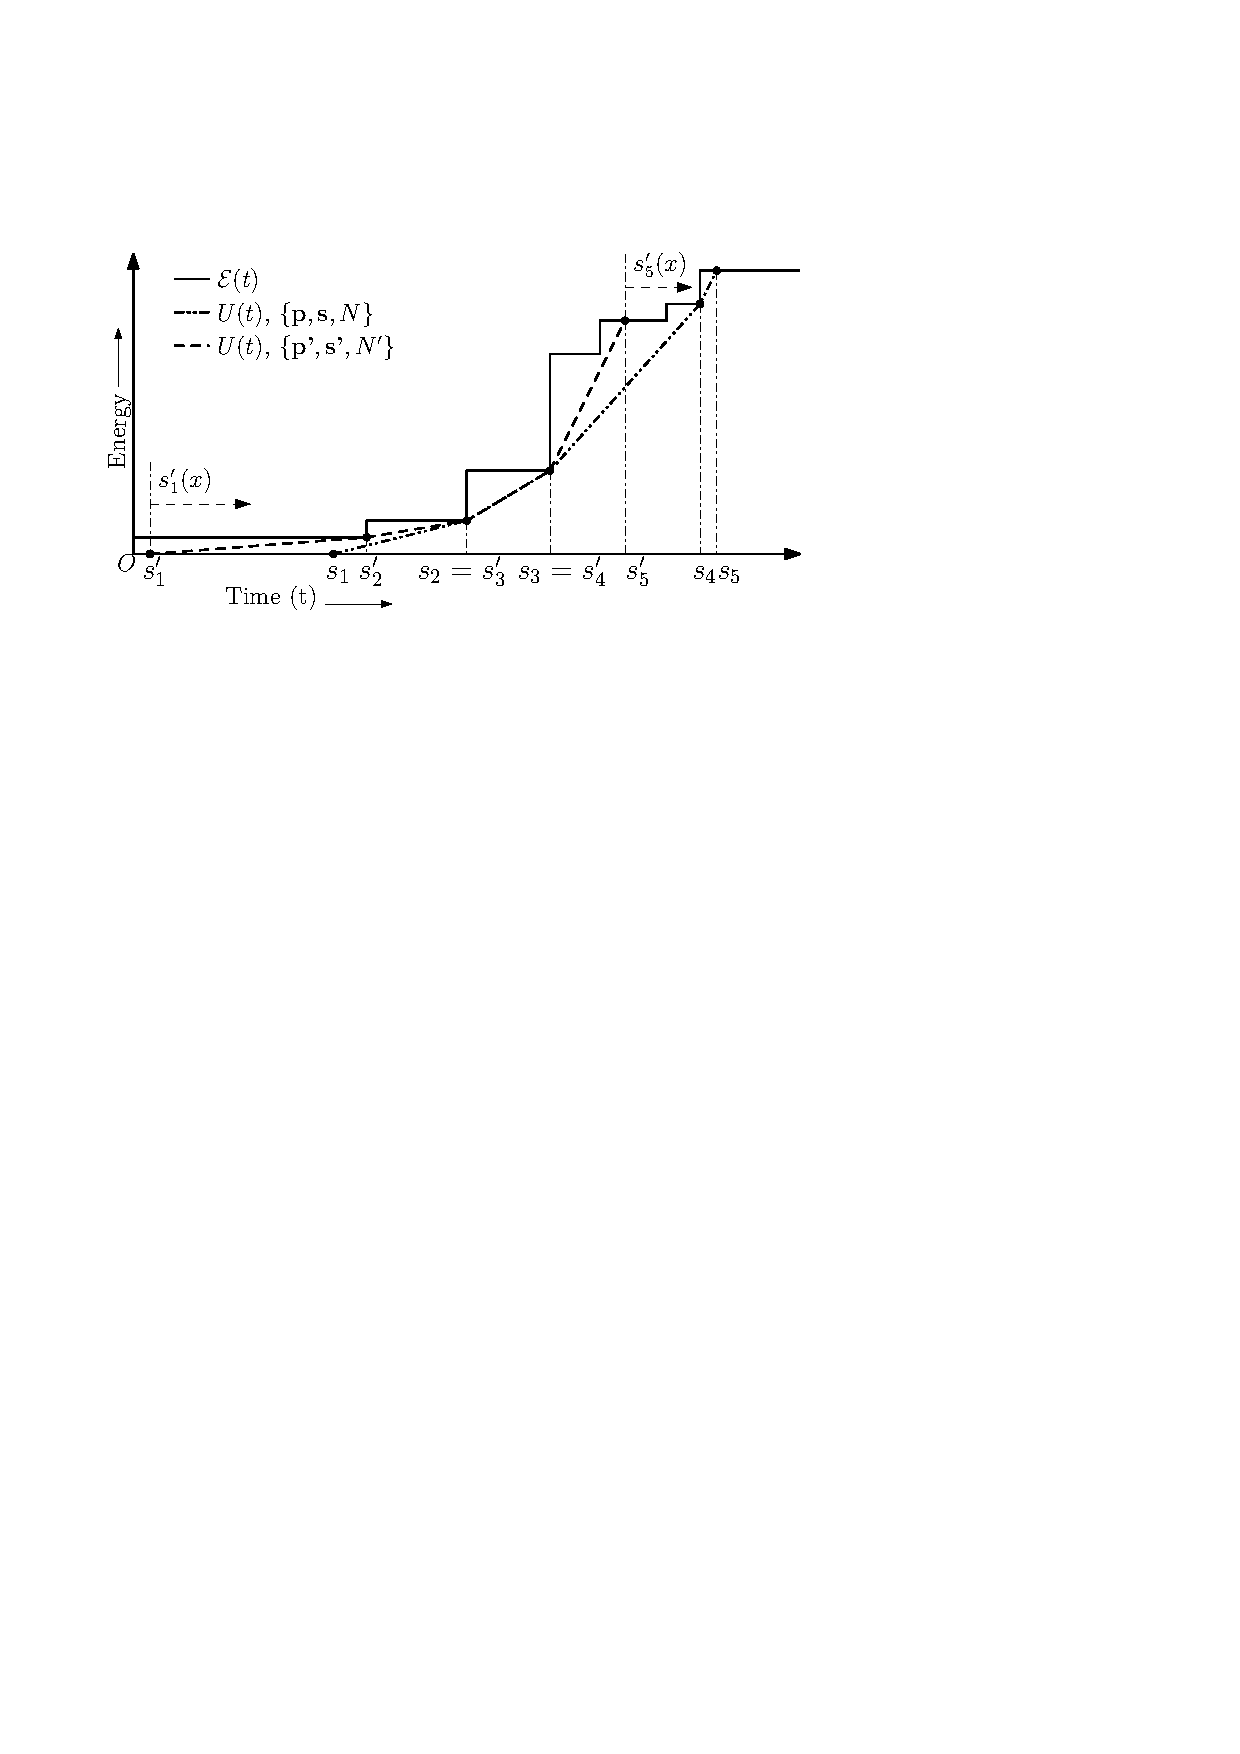
\includegraphics[width=8cm]{Theorem1_sufficient.pdf}}
\caption{Energy curves at Transmitter explaining \textit{Case3} in proof of Theorem \ref{th_algo1_1}}
\label{Theorem1_figure}
\end{figure}

Now, consider the following process which creates child feasible policies from policy $\{\textbf{p'},\textbf{s'},N'\}$ as shown in Figure \ref{Theorem1_figure}. We define two pivots $pv_1$ and $pv_2$. Initially we set $pv_1=s_2'$ and $pv_2=s_{N'}'$. The transmission power right before $pv_1$ is $u$ ($u=p_1'$ initially) and right after $pv_2$ is $v$ ($v=p_{N'}'$ initially). Keeping the policy same from $pv_1$ to $pv_2$ we increase $u$ by a small amount to $u+du$ and decrease $v$ by a small amount to $v-dv$ such that the number of bits transmitted ( i.e. $B_0$) remains same under this transformation. Let $s_1'$ change to $s_1'+x$ and $s_{N'+1}'$ change to $s_{N'+1}'+y$ for some $x,y>0$. We denote such a policy by vectors $\{\textbf{p'(x)},\textbf{s'(x)},N'(x)\}$. Following the argument provided while proving the necessary statement of this Theorem, we can conclude that $(s_{N'(x)+1}'(x)-s_1'(x))<(s_{N'+1}'-s_1')$. We continue increasing $x$ till either $u=p_2$ (in which case we change $pv_1=s_2$) or $v=p_{N'-1}'$ (where we change $pv_2=s_{N'-1}'$) or $s_{N'(x)+1}'(x)$ hits an epoch, say $t_j$ ($pv_2=t_j$, $v\rightarrow\infty$ in this case). After this, we again start increasing $x$ with changed definitions. We continue this process till $x=s_1-s_1'$  or $u$ becomes equal to $v$. Note that the former stopping criteria will be met at a smaller $x$ than the later one since policy $\{\textbf{p'(x)},\textbf{s'(x)},N'(x)\}$ shares at least one epoch with policy $\{\textbf{p},\textbf{s},N\}$ by arguments of previous paragraph. By maintaining these rules we ensure that policy $\{\textbf{p'(x)},\textbf{s'(x)},N'(x)\}$ abides by Lemma 1-5 and is feasible with energy constraint. Since $\left( s_{N'(x)+1}'(x)-s_1'(x)\right)$ is decreasing with $x$, the policy is also feasible with time constraint. As this is continuous on $x$, at $x=s_1-s_1'$ we reach a policy such that $s_1'(x)=s_1$. For $x=s_1-s_1'$, if $s_{N'(x)+1}'(x)\ge s_{N+1}$ then $s_{N'+1}'-s_1'>s_{N'(x)+1}'(x)-s_1'(x)\ge \TRx_0$ and policy $\{\textbf{p'},\textbf{s'},N'\}$ is infeasible with time constraint. If $s_{N'(x)+1}'(x)< s_{N+1}$ then we can follow the arguments in \textit{Case2} to show that policy $\{\textbf{p'(x)},\textbf{s'(x)},N'(x)\}$ is infeasible, which in turn accounts for the infeasibility of policy $\{\textbf{p'},\textbf{s'},N'\}$.
\end{proof}

























%input{Rushil}
\begin{theorem}
The policy described by the above algorithm is optimal.
\end{theorem}
\begin{proof}
To prove that our policy is optimal, we have to show that it is of the structure described in the previous theorem. \\
First we prove that the power allocations in this algorithm are in accordance with \eqref{claim3}\\
In the first part of the algorithm, we select the maximum slope at a corner point before $t_{lt}$ and after $t'_{start}$ and ending at $t_{lt}$. \\
First we try to show that this is also the maximum such slope between any corner point before $t_{lt}$ and after $t_{start}$ where $t_{start}$ is the final start point. \\
Suppose it is not. Then we have a corner point between $t_{start}$ and $t'_{start}$ such that we can transmit with a power higher than our maximum between these two points. But, if this were possible, then 
$p_{lt}$ itself would have been feasible, which is not the case. (See figure).\\
Now we seek to show that this procedure of selecting maximum slopes going 'backwards' also gives us the minimum slopes going 'forwards', as described in \eqref{claim3}.\\
We shall show this by contradiction. Let $t_i$, $t_j$ and $t_k$ be three consecutive corner points where the power of transmission increases, as per our allocation. Now suppose, it is possible to transmit with a lowe power between $t_i$ and some $t'_j$. 
Then the power of transmission between $t_j$ and $t_k$ is not the maximum power since we could transmit at a higher power from $t'_j$ and $t_k$. Which is a contradiction as this is not consistent with out allocation algorithm.\\
Therefore, the allocation policy before point $Q$ is consistent with the structure.. (See figure)
We can prove similarly for the powers after point $Q$.
\end{proof}




